%%%
% set up document type
%%%
\documentclass[12pt]{article}

%%%
% declare all packages
%%%
\usepackage[left=25mm, top=20mm, right=25mm, bottom=30mm,nohead,nofoot]{geometry} 

\usepackage[T2A]{fontenc}
\usepackage[utf8]{inputenc}
\usepackage[english, russian]{babel}

\usepackage{graphics, graphicx}

\usepackage{url}
\usepackage{hyperref}

\usepackage{amssymb,latexsym} 
\usepackage{MnSymbol}
\usepackage{mathrsfs}

\usepackage[nottoc,numbib]{tocbibind}
\usepackage{float}
\usepackage{listings}
\usepackage{multirow}
\usepackage{hhline}
\usepackage{delarray}

\usepackage{color,colortbl}

% \usepackage{verbatim}
%%%
% document settings
%%%
\setcounter{tocdepth}{4}
\graphicspath{ {./pic/} }

\renewcommand{\listoffigures}{\begingroup  % add number to list of graphics
\tocsection
\tocfile{\listfigurename}{lof}
\endgroup}
\renewcommand{\listoftables}{\begingroup  % add number to list of tables
\tocsection
\tocfile{\listtablename}{lot}
\endgroup}

\newcommand{\RomanNum}[1]
    {\MakeUppercase{\romannumeral #1}}

%******************************************************************
%******************************************************************
\begin{document}

\begin{titlepage}
	\center
		Санкт-Петербургский Политехнический 
		университет \\ Петра Великого\\
		Институт прикладной математики и механики
		\\ \textbf{Высшая школа прикладной математики и вычислительной физики}

	\vfill ~
	\textbf{
		\\ \large РАСЧЁТНОЕ ЗАДАНИЕ №1
	}
	\\	на тему 
	\\ "Исследование устойчивости системы"
	\\ по дисциплине
	\\ "Математическая теория управления"
    \\ \textbf{вариант №3}
	\vfill ~
    
    
    \begin{flushleft}
    \underline{Выполнил:}  \hspace{\fill} студент гр.3630102/60101 \textbf{Лансков.Н.В.} \linebreak[2]
	\underline{Руководитель:} \hspace{\fill} доцент \textbf{Суханов А.А.} \\ 
    \end{flushleft}
    

\vfill

{\large}	Санкт-Петербург
\\ 2020
\end{titlepage}

%%%
% Table of conetnts 
%%%

\tableofcontents 
\listoffigures
\pagebreak
% \listoftables
% \newpage

%%%
% Text
%%%
\section{Постановка задачи}
Дана передаточная функция для разомкнутой цепи:

\begin{equation}
 H_{r} = \dfrac{K(T_1p + 1)}{p(p^2+\omega_0^2)(T_2p + 1)(T_3p + 1)}
\end{equation}

где:

\begin{equation}
\begin{cases}
 K = 0.75 \\
 \omega_0 = 3 \\
 T_1 = 0.01 \\ 
 T_2 = 0.06 \\ 
 T_3 = 0.03 \\ 
\end{cases}
\end{equation}

Необходимо определить устойчивость системы с данной передаточной функцией, используя:
\begin{enumerate}
 \item Алгебраический критерий Льенара-Шепара
 \item Частотный критерий Михайлова
 \item Частотный критерий Найквиста
\end{enumerate}

\section{Решение}
\subsection{Критерий Льенара-Шепара}

Запишем формулу для передаточной функции замкнутой цепи:
\begin{equation}
 H_{z} = \dfrac{H_{r}}{1 + H_{r}} = \dfrac{K(T_1p + 1)}{K(T_1p + 1) + p(p^2+\omega_0^2)(T_2p + 1)(T_3p + 1)}
\end{equation}

Нас интересует знаменатель, рассмотрим его отдельно:

\begin{eqnarray}
 \alpha(p) = K(T_1p + 1) + p(p^2+\omega_0^2)(T_2p + 1)(T_3p + 1) = \nonumber \\ 
 = K + (T_2 + T_3)p^4 + p\omega_0^2 + p^3 + (T_2 + T_3)p^2\omega_0^2 + KT_1p + T_2T_3p^5 + T_2T_3p^3\omega_0^2 = \nonumber \\
 = p^5(T_2T_3) + p^4(T_2 + T_3) + p^3(1 + T_2T_3\omega_0^2) + p^2(T_2\omega_0^2 + T_3\omega_0^2) + p(\omega_0^2 + KT_1) + K
\end{eqnarray}

Запишем матрицу Гурвица:

$$
\begin{bmatrix}
 T_2 + T_3 & T_2\omega_0^2 + T_3\omega_0^2 & K & 0 & 0 \\
 T_2T_3 & 1 + T_2T_3\omega_0^2 & \omega_0^2 + KT_1 & 0 & 0\\
 0 & T_2 + T_3 & T_2\omega_0^2 + T_3\omega_0^2 & K & 0  \\
 0 & T_2T_3 & 1 + T_2T_3\omega_0^2 & \omega_0^2 + KT_1 & 0 \\
 0 & 0 & T_2 + T_3 & T_2\omega_0^2 + T_3\omega_0^2 & K \\
\end{bmatrix}
$$

\pagebreak
Проверим, выполняются ли условия критерия:
\begin{enumerate}
 \item $a_i > 0$ \\
 В силу того, что все коэффициенты в условии положительны, это требование очевидно выполнено.
 \item Нечётные(или чётные) главные миноры должны быть положительны \\ 
 $\Delta_1 > 0$ - очевидно из первого пункта \\
 $\Delta_3 = -0.0006074999999999829 < 0$ $\Rightarrow$ данное требование не выполнено, и, как следствие, согласно алгебраическому критерию система неустойчива.
 
\end{enumerate}


\subsection{Критерий Михайлова}

Для того, чтобы применить критерий Михайлова, необходимо построить характеристический полином:
\begin{equation}
 \alpha(j\omega) = jKT_1\omega + K + jT_2T_3\omega^5 - jT_2T_3\omega^3\omega_0^2 + T_2\omega^4 - 
 T_2\omega^2\omega_0^2 + T_3\omega^4 - T_3\omega^2\omega_0^2 - j\omega^3 + j\omega\omega_0^2
\end{equation}
Данный полином представляет собой комплекснозначную функцию. Выпишем вещественную и мнимую части:
\begin{equation}
 \begin{cases}
  Re(\alpha(j\omega)) = K + (T_2 + T_3)\omega^4 - (T_2 + T_3)\omega^2\omega_0^2 \\
  Im(\alpha(j\omega)) = KT_1\omega + T_2T_3\omega^5 -T_2T_3\omega^3\omega_0^2 - \omega^3 + \omega\omega_0^2
 \end{cases}
\end{equation}

Построим зависимость мнимой части от вещественной, задав некоторый шаг по $\omega$

\begin{figure}[H]
\centerline{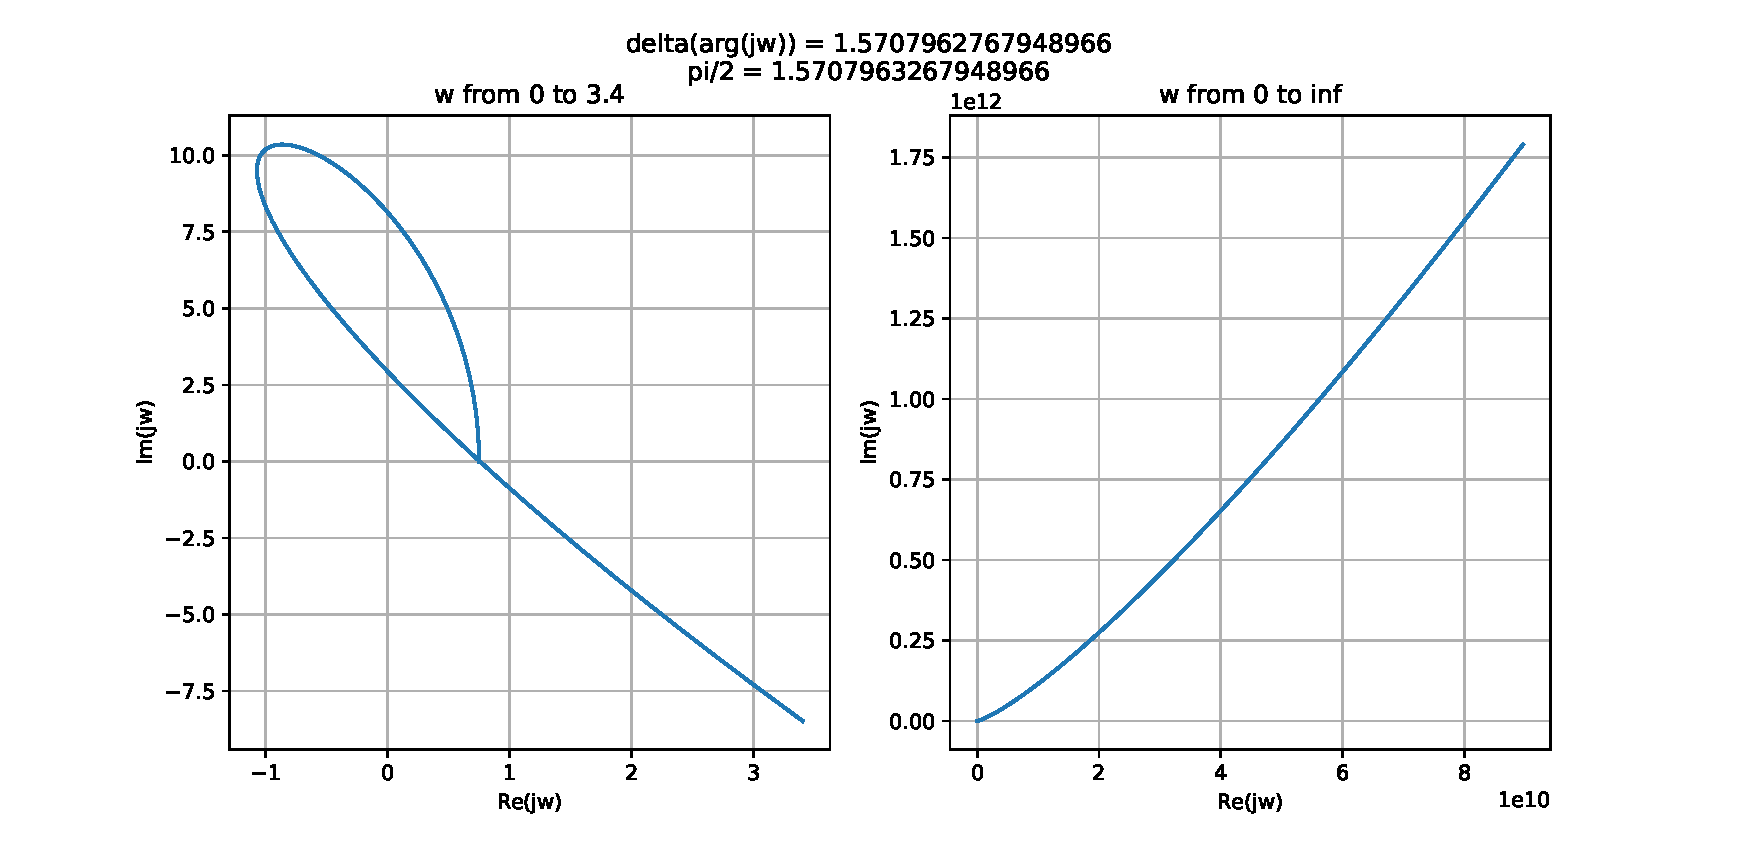
\includegraphics[scale = 0.6]{Figure_1.eps}}
\caption{Вид кривой Михайлова}
\end{figure}

\pagebreak

По графику видно, что вектор кривой не оборачивается вокруг нуля. Чтобы система была устойчивой, построенный график должен лежать в пяти квадрантах (\RomanNum{1}, \RomanNum{2}, \RomanNum{3}, \RomanNum{4}, \RomanNum{1}(\RomanNum{5})), что в данном случае не выполняется. Кроме аппеляции к графику, можно также рассматривать значение $\Delta arg(\alpha(j\omega))$, которое в данном случае равняется $1.570796 \xrightarrow[\omega \rightarrow \infty]{} \dfrac{\pi}{2} $. Таким образом, системя не является устойчивой согласно данному критерию.

\subsection{Критерий Найквиста}

Исследуем аналогично предыдущему пункту годограф функции вида:

\begin{equation}
 \psi(j \omega) = 1 + H_{r}(j \omega) 
\end{equation}

\begin{figure}[H]
\centerline{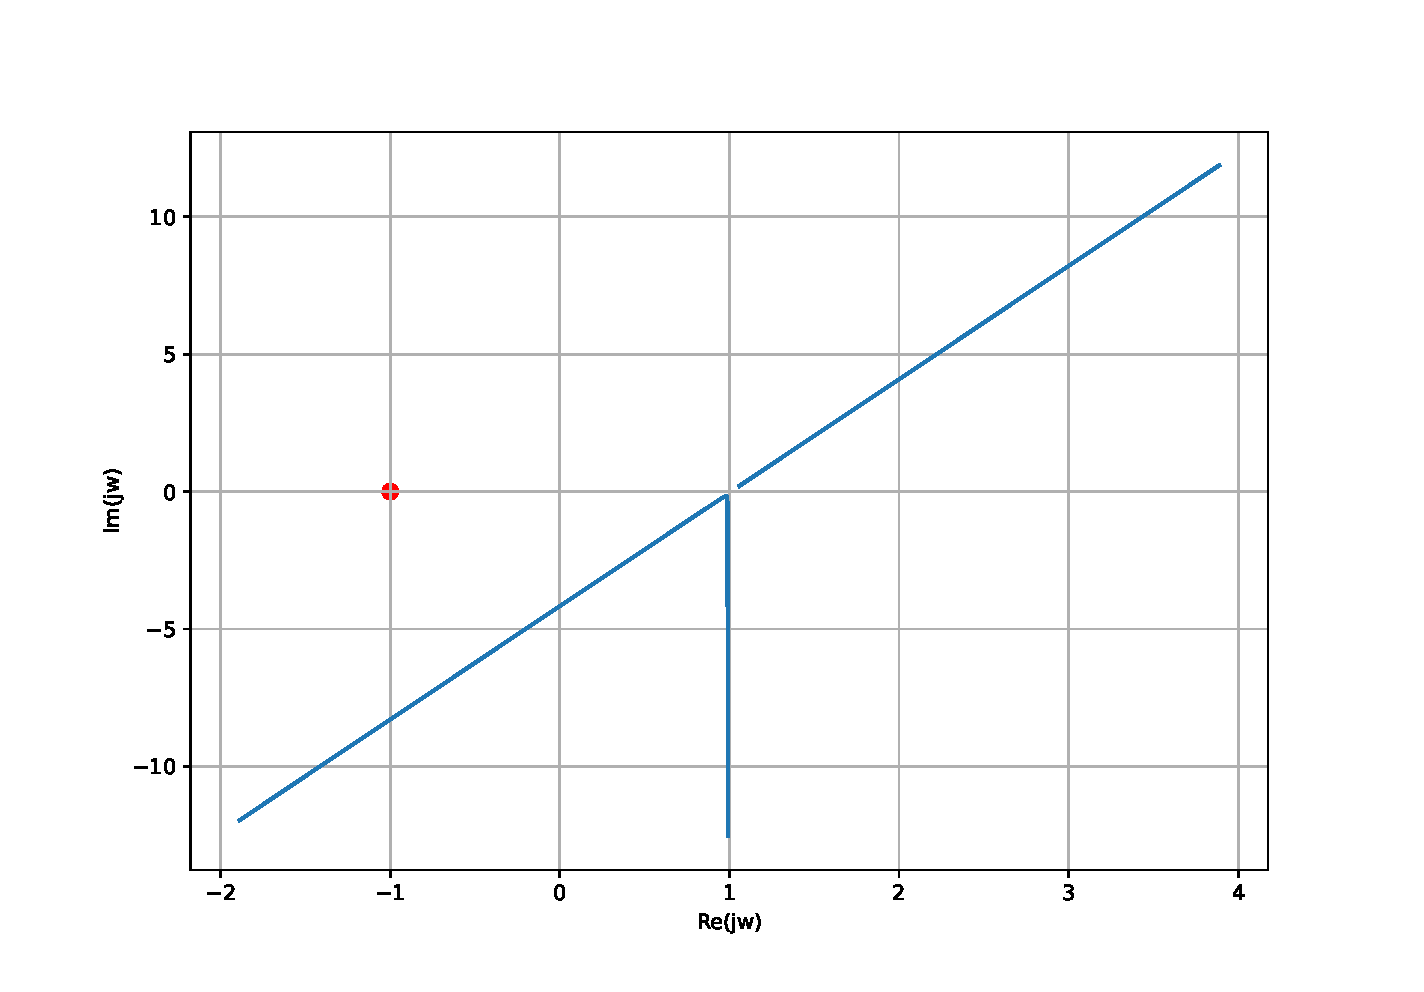
\includegraphics[scale = 0.6]{Figure_2.eps}}
\caption{Вид кривой Найквиста}
\end{figure}

Из графика видно, что годограф `охватывает` точку (-1, 0j). Отсюда следует, что исследуемая система является неустойчивой.

\section{Результаты}

В результате проведённых исследований, заданная система оказалась неустойчивой согласно всем трём использованным критериям

\end{document}

